\chapter{Исследовательский раздел}

В данном разделе будут приведены: пример работы программы, постановка эксперимента и сравнительный анализ алгоритмов на основе полученных данных.

\section{Демонстрация работы программы}


На рисунке \ref{img:program} представлена демонстрация работы разработанного программного обеспечения, а именно показаны результаты сортировки массива $[3, 5, -3, 1, 2, 4, -6, 2]$.

\includeimage
{program} % Имя файла без расширения (файл должен быть расположен в директории inc/img/)
{f} % Обтекание (без обтекания)
{h} % Положение рисунка (см. figure из пакета float)
{0.65\textwidth} % Ширина рисунка
{Демонстрация работы программы при сортировке массива} % Подпись рисунка

\clearpage


\section{Технические характеристики}

Технические характеристики компьютера, на котором проводился замерный эксперимент:
\begin{itemize}
	\item процессор Intel Core i5-10400F (6 ядер) \cite{intel};
	\item 16 Гб оперативная память DDR4;
	\item операционная система Windows 10 Pro \cite{windows}.
\end{itemize}

Во время проведения исследования компьютер был нагружен только системными приложениями и целевой программой.

\section{Время выполнения реализаций алгоритмов}

Результаты замеров времени выполнения реализаций алгоритмов сортировок приведены в таблицах \ref{tbl:time_measurements} -- \ref{tbl:time_measurements_rand}.
Замеры времени проводились на массивах одного размера и усреднялись для каждого набора одинаковых экспериментов.

В таблицах \ref{tbl:time_measurements} -- \ref{tbl:time_measurements_rand} используются следующие обозначения: 
\begin{itemize}
	\item Блочная --- реализация алгоритма блочной сортировки;
	\item Быстрая --- реализация алгоритма быстрой сортировки;
	\item Выбором --- реализация алгоритма сортировки выбором.
\end{itemize}

\begin{table}[h]
	\begin{center}
		\begin{threeparttable}
			\captionsetup{justification=raggedright,singlelinecheck=off}
			\caption{Время работы реализации алгоритмов на неотсортированных массивах (в мс)}
			\label{tbl:time_measurements}
			\begin{tabular}{|c|c|c|c|}
				\hline
				Размер массива & Блочная & Быстрая & Выбором \\
				\hline
				100 &$ 0.078125 $&$ 0.125 $&$ 0.203125 $\\
				\hline
				200 &$ 0.203125 $&$ 0.265625 $&$ 0.90625 $\\
				\hline
				300 &$ 0.40625 $&$ 0.5 $&$ 1.78125 $\\
				\hline
				400 &$ 0.765625 $&$ 0.546875 $&$ 3.484375 $\\
				\hline
				500 &$ 1.078125 $&$ 0.734375 $&$ 5.625 $\\
				\hline
				600 &$ 1.390625 $&$ 0.890625 $&$ 7.8125 $\\
				\hline
				700 &$ 1.8125 $&$ 1.15625 $&$ 10.609375 $\\
				\hline
				800 &$ 2.234375 $&$ 1.25 $&$ 14.25 $\\
				\hline
				900 &$ 2.984375 $&$ 1.296875 $&$ 18.0625 $\\
				\hline
				1000 &$ 3.734375 $&$ 1.5 $&$ 22.515625 $\\
				\hline
			\end{tabular}
		\end{threeparttable}
	\end{center}
\end{table}

\begin{table}[h]
	\begin{center}
		\begin{threeparttable}
			\captionsetup{justification=raggedright,singlelinecheck=off}
			\caption{Время работы реализации алгоритмов на отсортированных в обратном порядке массивах (в мс)}
			\label{tbl:time_measurements_sorted}
			\begin{tabular}{|c|c|c|c|}
				\hline
				Размер массива & Блочная & Быстрая & Выбором \\
				\hline
				100 &$ 0.078125 $&$ 0.125 $&$ 0.203125 $\\
				\hline
				200 &$ 0.203125 $&$ 0.25 $&$ 0.765625 $\\
				\hline
				300 &$ 0.40625 $&$ 0.390625 $&$ 1.9375 $\\
				\hline
				400 &$ 0.640625 $&$ 0.546875 $&$ 3.3475 $\\
				\hline
				500 &$ 0.96875 $&$ 0.6875 $&$ 5.375 $\\
				\hline
				600 &$ 1.328125 $&$ 0.875 $&$ 7.609375 $\\
				\hline
				700 &$ 1.75 $&$ 1.046875 $&$ 10.640625 $\\
				\hline
				800 &$ 2.609375 $&$ 1.140625 $&$ 14.046875 $\\
				\hline
				900 &$ 2.9375 $&$ 1.25 $&$ 17.828125 $\\
				\hline
				1000 &$ 3.71875 $&$ 1.4375 $&$ 22.265625 $\\
				\hline
			\end{tabular}
		\end{threeparttable}
	\end{center}
\end{table}

\begin{table}[h]
	\begin{center}
		\begin{threeparttable}
			\captionsetup{justification=raggedright,singlelinecheck=off}
			\caption{Время работы реализации алгоритмов на отсортированных массивах (в мс)}
			\label{tbl:time_measurements_rand}
			\begin{tabular}{|c|c|c|c|}
				\hline
				Размер массива & Блочная & Быстрая & Выбором \\
				\hline
				100 &$ 0.0625 $&$ 0.109375 $&$ 0.203125 $\\
				\hline
				200 &$ 0.203125 $&$ 0.3125 $&$ 0.828125 $\\
				\hline
				300 &$ 0.390625 $&$ 0.4375 $&$ 1.859375 $\\
				\hline
				400 &$ 0.640625 $&$ 0.578125 $&$ 3.453125 $\\
				\hline
				500 &$ 1 $&$ 0.6875 $&$ 5.3125 $\\
				\hline
				600 &$ 1.3125 $&$ 0.859375 $&$ 7.90625 $\\
				\hline
				700 &$ 1.890625 $&$ 1.03125 $&$ 10.46875 $\\
				\hline
				800 &$ 2.28125 $&$ 1.125 $&$ 13.8125 $\\
				\hline
				900 &$ 2.9375 $&$ 1.3125 $&$ 18.109375 $\\
				\hline
				1000 &$ 3.4375 $&$ 1.4375 $&$ 22.421875 $\\
				\hline
			\end{tabular}
		\end{threeparttable}
	\end{center}
\end{table}

\clearpage
На рисунках \ref{pic:random} -- \ref{pic:sorted} изображены графики зависимостей времени выполнения реализаций сортировок от размеров массивов.

\begin{figure}[H]
	\centering
	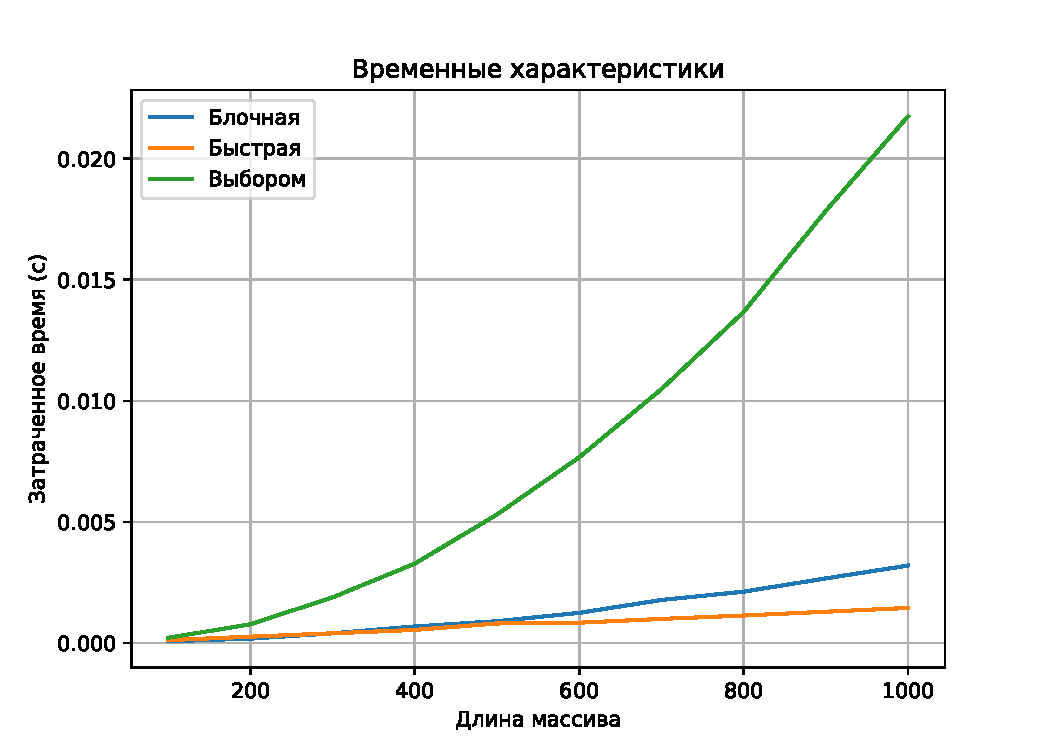
\includegraphics[scale=0.62]{assets/plots/cpu-random.pdf}
	\caption{Сравнение реализаций алгоритмов по времени выполнения на неотсортированных массивах}
	\label{pic:random}
\end{figure}

\newpage

\begin{figure}[H]
	\centering
	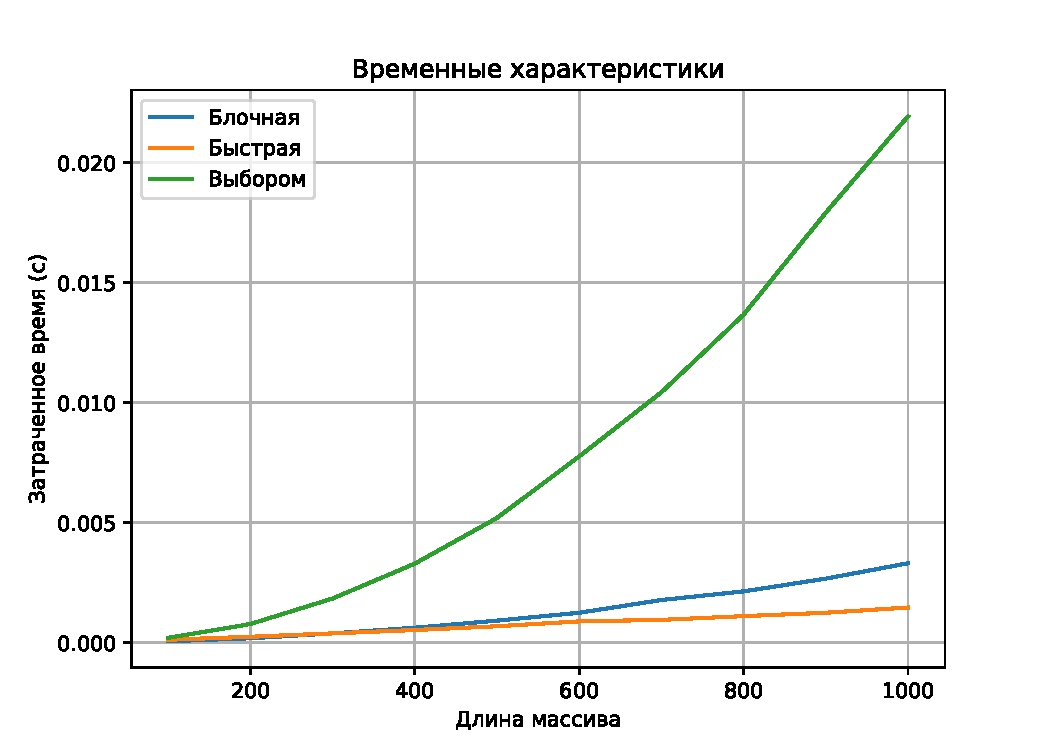
\includegraphics[scale=0.62]{assets/plots/cpu-reversed.pdf}
	\caption{Сравнение реализаций алгоритмов по времени выполнения на отсортированных в обратном порядке массивах}
	\label{pic:reversed}
\end{figure}

\newpage

\begin{figure}[H]
	\centering
	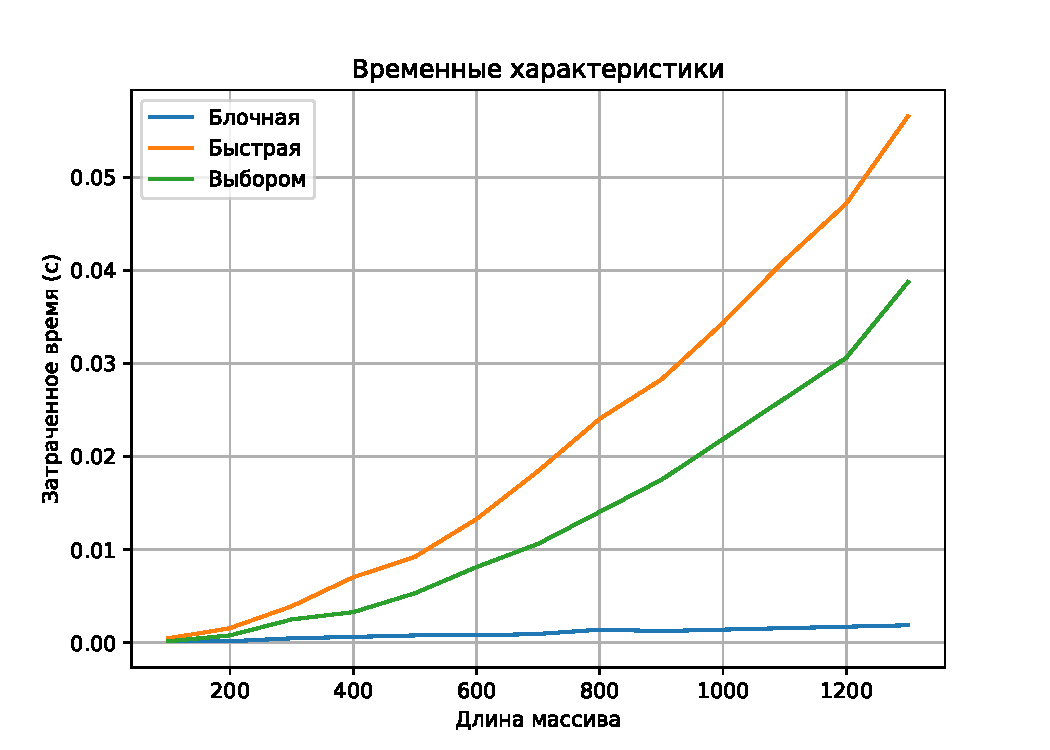
\includegraphics[scale=0.62]{assets/plots/cpu-sorted.pdf}
	\caption{Сравнение реализаций алгоритмов по времени выполнения на отсортированных массивах}
	\label{pic:sorted}
\end{figure}

\clearpage


\section*{Вывод}

В результате замеров времени выполнения реализаций различных алгоритмов было выявлено, что для массивов длины 1000, отсортированных в обратном порядке, реализация алгоритма быстрой сортировки по времени оказалась в 2.59 раз лучше, чем реализация блочной сортировки, и в 15.49 раз лучше реализации сортировки выбором. 
В свою очередь, реализация блочной сортировки оказалась лучше в 5.99 раз по времени выполнения, чем реализация  сортировки выбором.

Для отсортированных массивов длиной 1000 реализация быстрой сортировки оказалась лучше по времени в 2.39 раз, чем реализация блочной сортировки, и в 15.6 раз лучше, чем реализация сортировки выбором. 
В свою очередь, реализация блочной сортировки оказалась лучше в 6.52 раз по времени выполнения, чем реализация сортировки выбором.

Для случайно упорядоченных массивов длиной 1000 реализация быстрой сортировки оказалась лучше по времени в 2.49 раз, чем реализация блочной сортировки, и в 15.01 раза лучше, чем реализация сортировки выбором. 
В свою очередь, реализация блочной сортировки на случайно упорядоченных массивах оказалась лучше в 6.03 раза по времени выполнения, чем реализация сортировки выбором.

Стоит заметить, что для массивов длиной менее 300, реализация блочной сортировки была лучше или такой же по времени выполнения по сравнению с быстрой сортировкой, но на массивах ллины более 300 быстрая сортировка становилась лучше по времени выполнению.